\documentclass{article}
\usepackage{amsmath}
\usepackage{graphicx}
\usepackage{../../raccourcis}

\newcommand{\nom}{TD8 : Modulation et démodulation FM pour la vidéo}
\renewcommand{\nomentete}{UE431 - \nom}

\begin{document}

\titre{\nom}

On effectue les hypothèses suivantes : 
\begin{itemize}
\item Les deux signaux $\left \{\begin{matrix}d_r(t) \text{	transmis en FM à $f_r$ avec } \Delta f_r = 280kHz\\d_b(t) \text{	transmis en FM à $f_b$ avec } \Delta f_b = 230kHz\end{matrix} \right.$\\
\item Modulante FM de constante caractéristique $k_f$ ($Hz.V^{-1}$)
\item $\left \{\begin{matrix}d_r(t)\\d_b(t)\end{matrix} \right.$ de spectre inclut dans $[0;B_0 = 2MHz]$
\end{itemize}
\bigbreak

\begin{enumerate}
\item \begin{align*}
s_r(t) &= A_2 cos(2\pi f_rt + \phi_r(t))
\text{ avec }\left \{ \begin{matrix}
\Phi_r(t) = 2 \pi f_r t + \phi_r(t)\\
\phi_r(t) = \text{dérivation en phase}
\end{matrix} \right.
\intertext{La fréquence instantanée est :}
f_i(t) &= \frac{1}{2\pi}\frac{d \Phi(t)}{dt}\\
&= f_r + \frac{1}{2\pi} \frac{df_r(t)}{dt}
\intertext{La dérivation de phase instantanée est donc :}
\Delta f(t) &= \frac{1}{2\pi}\frac{df_r(t)}{dt}
\intertext{De plus, on a $\Delta f(t) = k_f d_r(t)$, d'où :}
s_r(t) &= A_2 cos(2\pi f_rt + 2\pi k_f \int_0^td_r(u)du)
\end{align*}

L'excursion en fréquence est alors $|\Delta f|_{max} = \Delta f_r$

\item Déterminons l'indice de modulation $\beta_r$ :
\begin{align*}
\beta &= \frac{\text{excursion en fréquence}}{\text{frequence max du modulant}}
\beta_r &= \frac{\Delta f_r}{B_0}
\end{align*}

\begin{center}
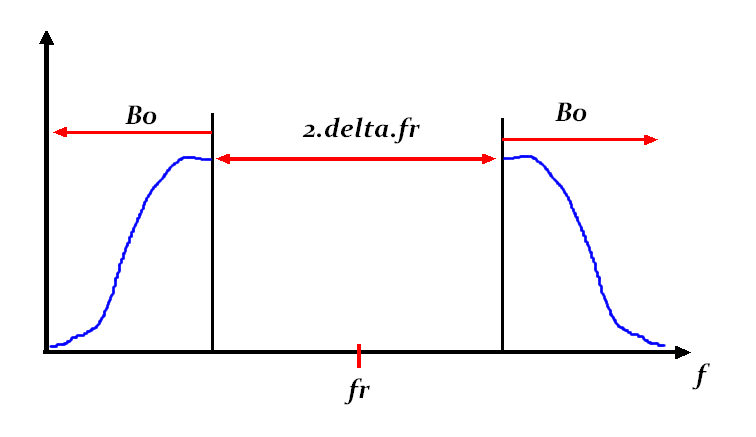
\includegraphics[scale=0.5]{TD9-1.png}
\end{center}

\item Determinons l'encombrement en frequence $B_{ur}$ :
\paragraph{Règle de Carson }:\\
L'encombrement utile en fréquence d'une modulation FM est :
\[B_{ur} = 2B_0(1+\beta) = 2(B_0 + \Delta f_r) = 4.56MHz\]

\item Quand la PLL est accrochée, les fréquences instantanées des signaux d'entrée et de sortie de la PLL sont égales donc :
\[f_e(t) = f_r + k_rd_r(t)\]

\item Où retrouve-t-on le signal modulant?
 on a :
 \begin{align*}
 f_e(t) &= f_r + k_{VCO} v_m(t)
 \intertext{or,}
 f_e(t) &= f_r + k_rd_r(t)
 \intertext{d'où,}
 v_m(t) &= \frac{k_rd_r(t)}{k_{VCO}}
 \end{align*}
 On retrouve le signal modulant en entrée du VCO.
 
 \item Il faut que la caractéristiqu $f_e(t) = f_r + k_{VCO} v_m$ soit linéaire sur l'intervalle $[f_r-\Delta f_r ; f_r + \Delta f_r]$\\
 
 \item Le schéma bloc associé est :
 
 \begin{center}
% 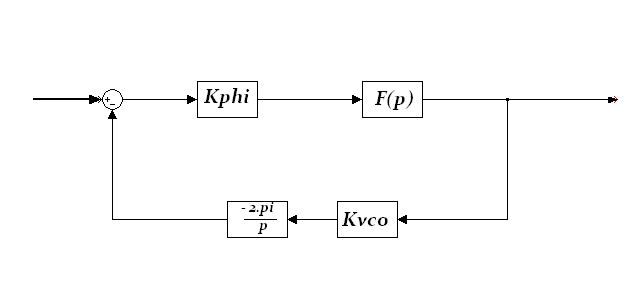
\includegraphics[scale=0.5]{TD9-2.png}
 \end{center}

\item 
On commence par exprimer avec la formule de Black : $\frac{V_m(p)}{\Phi_{sr}(p)} = \frac{K_{\Phi}F(p)}{1 + K_{\Phi}F(p)K_{VCO}\frac{2\pi}{p}}$\\
$\Phi_{sr}(t)$ est tel que $f_{sr}(t) = \frac{1}{2\pi}\frac{d\Phi_{sr}(t)}{dt}$\\
Après transformée de Laplace, on a :
\begin{align*}
F_{sr}(p) &= \frac{1}{2\pi}p\Phi_{sr}(p) \Rightarrow \Phi_{sr}(p) = \frac{2\pi}{p}F_{sr}(p)
\intertext{d'où :}
\frac{V_m(p)}{F_{sr}(p)} &= \frac{K_{\Phi} F(p) \frac{2\pi}{p}}{1 + K_{\Phi}F(p)K_{VCO}\frac{2\pi}{p}}
\end{align*}

On fait l'hypothèse que les deux filtre passses bas sont envisagées avec :\\
cas 1 : $T_{01}(p) = \frac{2\pi K_{\Phi} K_{VCO}}{p(1+RCp}$\\
cas 2 : $T_{02}(p) = 2\pi K_{\Phi} K_{VCO} \frac{1+RCp}{R_2Cp^2}$

\item Ammortissement $\xi$ et bande passante $f_BF$ de la PLL\\

Exprimons la FTBF pour le filtre F1
\begin{align*}
\frac{V_m(p)}{F_r(p)} &= \frac{1}{K_{VCO}} \frac{1}{1+\frac{1}{2\pi K_{\Phi} K_{VCO}}p + \frac{RC}{2\pi K_{\Phi} K_{VCO}}p^2}
\intertext{On identifie :}
f_{BF} &= \sqrt{\frac{K_{\Phi} K_{VCO}}{2\pi RC}}\\
\xi &= \frac{1}{2} \frac{1}{\sqrt{2\pi K_{\Phi} K_{VCO} RC}}
\end{align*}
Exprimons la FTBF pour le filtre $F_2$ :
\begin{align*}
\frac{V_m(p)}{F_r(p)} &=\frac{K_{\Phi}(\frac{1+R_1Cp}{R_2Cp})\frac{2\pi}{p}}{1+K_{\Phi}\frac{1+R_1Cp}{R_2Cp}K_{VCO}\frac{2\pi}{p}}\\
&= \frac{\frac{(1+R_1Cp)}{K_{VCO}}}{1+R_1Cp + \frac{R_2Cp^2}{2\pi K_{\Phi}K_{VCO}}}\\
f_{BF} &= \sqrt{\frac{K_{\Phi} K_{VCO}}{2\pi R_2C}}\\
\xi &= \frac{R_1C}{2} \sqrt{\frac{2\pi K_{\Phi} K_{VCO} RC}{R_2C}}
\end{align*}
Conclusion : Il est plus facile de régler la PLL avec $F_2$, car on peut régler indépendemment $f_{BF}$ et $\xi$ via $R_2$ et $R_1$

\item 10 Réglage de $f_{BF}$
Il faut $f_{BF} > B_0$ pour que le signal informatif soit correctement restitué.\\

\item Erreurs de phase\\
\begin{align*}
\Phi_{\epsilon}(p) =& \Phi_{sr}(p)-\Phi_e(p)\\ 
& \vdots\\
=& \Phi_{sr}(p)\frac{1}{1+K_{\Phi}K_{VCO}F(p) \frac{2\pi}{p}}
\end{align*}
Si une rampe de phase (ie, un échelon de fréquence) est appliqué en entrée de la PLL, on a : $ \Phi_{sr}(p) = \frac{\Phi_0}{p^2}$\\
Pour le filtre $F_1$ on a,
\[\Phi_{\infty} = \frac{\Phi_0}{2\pi K_{\Phi} K_{VCO}}\]
Pour le filtre $F_2$ on a,
\[\Phi_{\infty} = 0\]

\item Conclusion : $F_2$ est plus intéressant et permet d'annuler l'erreur de phase.


\end{enumerate}
\end{document}
